\documentclass[12pt,letterpaper,oneside]{book}
\usepackage{astro-thesis}
\usepackage{lipsum}


\begin{document}
	\begin{titlepage}
		\begin{center}
			
\includegraphics[height=3cm]{img/sample_logo.pdf}
			
			\vspace{2cm}
			
			{\fontsize{25}{40}\selectfont \bf Title\par}
			
			\vspace{10mm}
			
			{\huge Author}
			
			\vspace{10mm}
			
			{\huge Second Author } 
			
			\vspace{15mm}
			
			{\large
				A thesis submitted in partial fulfillment\\
				for the degree of 
			}
			
			\vspace{5mm}
			
			{\Large
				University\\
				Faculty, Department\\
				City, Country\\ \phantom{} \\
				Date
			}
		\end{center}
	\end{titlepage}
    
    
\frontmatter 

\chapter*{Abstract}

\lipsum{3}


\newpage

\begin{flushright}
	\textit{
		My        \\
		Cheesy           \\
		words
	}
\end{flushright}

\vspace{2mm}

\chapter*{Acknowledgements}

\lipsum{4}

\mainmatter

\tableofcontents

\newpage

\listoffigures
\listoftables
\listoflistings

\newpage

\visibleintentfalse

\chapter{Introduction}
\lipsum{20}

\begin{figure}[H]
	\centering
	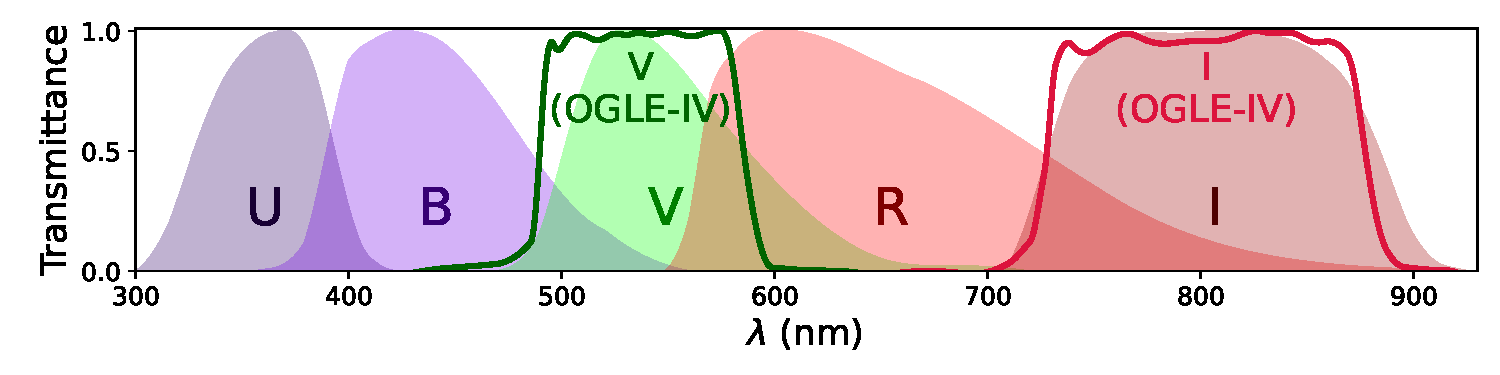
\includegraphics[width=\textwidth]{img/filters.pdf}
	\caption[Johnson-Cousins and OGLE-IV photometric systems]{
		Johnson-Cousins (filled) and OGLE-IV equivalent (solid) filters transmittance curves. 
		Colors are meant to be representative, not exact. UBVRI curves were adapted from \cite{Bessell2005}, and OGLE-IV curves from \cite{OGLE2015}. 
		It is to note that OGLE-IV curves are experimental measurements of custom made filters.
	}
	\label{fig:filters}
\end{figure}

\begin{table}
	\centering
	\begin{tabular}{c|c||c|c}
		Filter & description & $\lambda_{eff}$ (nm) & $\Delta_{\lambda}$ (nm) \\ \hline\hline
		U & Ultraviolet & 366.3 & 65 \\ 
		B & Blue & 436.1 & 89 \\ 
		V & Visual & 544.8 & 84 \\ 
		R & Red & 640.7 & 158 \\ 
		I & Infrared & 798 & 154
	\end{tabular}
	\caption[Johnson-Cousins effective wavelengths and bandwidths]{
		Effective wavelengths and bandwidths for the Johnson-Cousins photometric system. Data from \cite{Bessell2005}.
		}
	\label{tab:filters}
\end{table}

	
\chapter{Theoretical Framework}
\lipsum{20}

\chapter{Methodology}
\lipsum{20}

\chapter{Results}
\lipsum{20}

\chapter{Conclusions}
\lipsum{20}

% Bibliography

\nocite{*}%test

\bibliographystyle{aa_url} % style aa.bst
\bibliography{global.bib}

% Appendices

\appendix
\appendixpage
\noappendicestocpagenum
\addappheadtotoc

\chapter{Code utilities}
\lipsum{2}

\begin{listing}[H]
	\begin{minted}{c}
	double eps(double x) {
	    long i = *(long*) &x;
	    i++;
	    double x_next = *(double*) &i;
	    return x_next - x;
	}
	\end{minted}
	\caption[\texttt{eps} C function]{
		C code
	}
	\label{lst:c-eps}
\end{listing}

\lipsum{2}

\chapter{Complementary figures}
\lipsum{20}












\end{document}